%\documentclass[10pt]{article}
%\documentclass[crop,tikz,convert=pdf2svg]{standalone} %for an svg
\documentclass[%
  border={5pt 5pt 5pt 5pt}, % left bottom right top
  convert %=pdf2svg %for an svg
]{standalone}%

\usepackage{color}
\usepackage{tikz}
%%Source: https://dkumor.com/posts/technical/2018/08/15/causal-tikz/
% Tikz settings optimized for causal graphs.
% Just copy-paste this part
\usetikzlibrary{shapes,decorations,arrows,calc,arrows.meta,fit,positioning}
\tikzset{
    -Latex,auto,node distance =1 cm and 1 cm,semithick,
    state/.style ={ellipse, draw, minimum width = 0.7 cm},
    point/.style = {circle, draw, inner sep=0.04cm,fill,node contents={}},
    bidirected/.style={Latex-Latex,dashed},
    el/.style = {inner sep=2pt, align=left, sloped}
}
\begin{document}

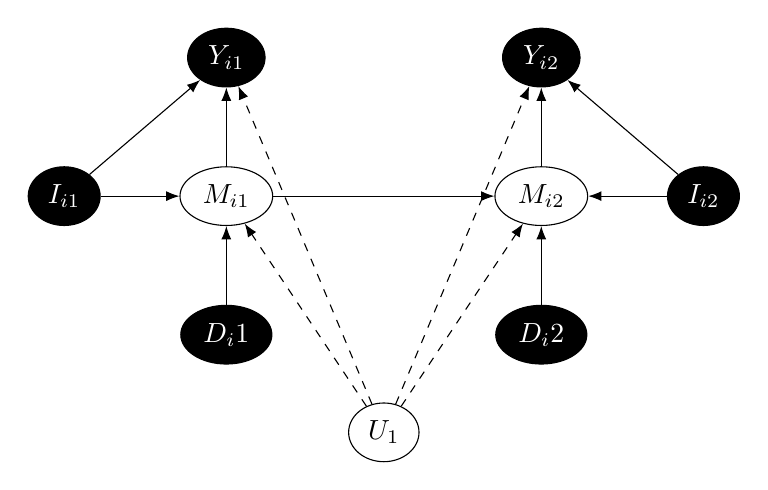
\begin{tikzpicture}
    % Unit 1

    %%Nodes
    \node[state, fill=black, text=white] (y1) at (-1,0) {$Y_{i1}$};
    \node[state] (m1) [below =of y1] {$M_{i1}$};
    \node[state, fill=black, text=white] (i1) [left =of m1] {$I_{i1}$};
    \node[state, fill=black, text=white] (d1) [below =of m1] {$D_i1$};
    \node[state] (u1) [below =of y1, yshift=-3cm, xshift=2cm] {$U_1$};]
     
	%%Nodes
	\node[state, fill=black, text=white] (y2) [above =of u1, yshift=3cm, xshift=2cm] {$Y_{i2}$};
    \node[state] (m2) [below =of y2] {$M_{i2}$};
    \node[state, fill=black, text=white] (i2) [right =of m2] {$I_{i2}$};
    \node[state, fill=black, text=white] (d2) [below =of m2] {$D_i2$};
   
     
    
    % Directed edge
    \path (m1) edge (y1);   
    \path (i1) edge (m1);
    \path (i1) edge (y1);
    \path (d1) edge (m1);
    \path (u1) edge[dashed] (y1);
    \path (u1) edge[dashed] (m1);
    
    \path (m2) edge (y2);   
    \path (i2) edge (m2);
    \path (i2) edge (y2);
    \path (d2) edge (m2);
    \path (u1) edge[dashed] (y2);
    \path (u1) edge[dashed] (m2);
    \path (m1) edge (m2);   
    
 
    
    
    
\end{tikzpicture}
\end{document}